\chapter{数据结构设计}
\section{用户管理系统数据结构设计}
需要学生个人信息表、教师信息表、科目信息表、开课结果信息表、成绩表

\section{物理结构设计}
无

\section{数据结构}
\begin{figure}[H] %H为当前位置,!htb为忽略美学标准,htbp为浮动图形
    \centering %图片居中
    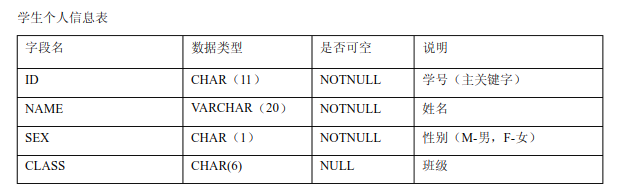
\includegraphics[width=0.7\textwidth]{选区_006} %插入图片,[]中设置图片大小,{}中是图片文件名
    \caption{学生个人信息表} %最终文档中希望显示的图片标题
    \label{Fig.main2} %用于文内引用的标签
\end{figure}

\begin{figure}[H] %H为当前位置,!htb为忽略美学标准,htbp为浮动图形
    \centering %图片居中
    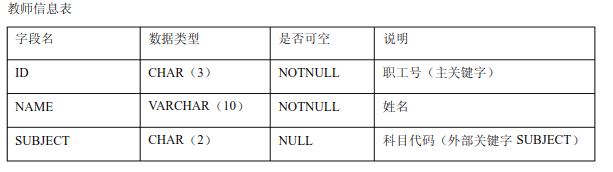
\includegraphics[width=0.7\textwidth]{选区_007} %插入图片,[]中设置图片大小,{}中是图片文件名
    \caption{教师信息表} %最终文档中希望显示的图片标题
    \label{Fig.main2} %用于文内引用的标签
\end{figure}

\begin{figure}[H] %H为当前位置,!htb为忽略美学标准,htbp为浮动图形
    \centering %图片居中
    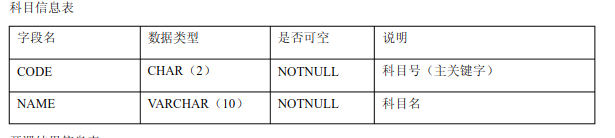
\includegraphics[width=0.7\textwidth]{选区_008} %插入图片,[]中设置图片大小,{}中是图片文件名
    \caption{科目信息表} %最终文档中希望显示的图片标题
    \label{Fig.main2} %用于文内引用的标签
\end{figure}

\begin{figure}[H] %H为当前位置,!htb为忽略美学标准,htbp为浮动图形
    \centering %图片居中
    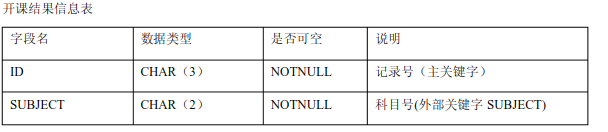
\includegraphics[width=0.7\textwidth]{选区_009} %插入图片,[]中设置图片大小,{}中是图片文件名
    \caption{开课结果信息表} %最终文档中希望显示的图片标题
    \label{Fig.main2} %用于文内引用的标签
\end{figure}

\begin{figure}[H] %H为当前位置,!htb为忽略美学标准,htbp为浮动图形
    \centering %图片居中
    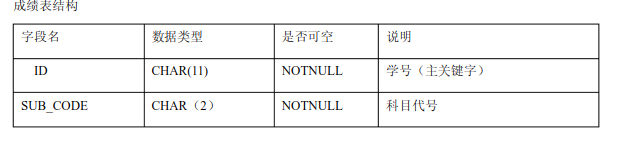
\includegraphics[width=0.7\textwidth]{选区_010} %插入图片,[]中设置图片大小,{}中是图片文件名
    \caption{成绩表} %最终文档中希望显示的图片标题
    \label{Fig.main2} %用于文内引用的标签
\end{figure}
